\section*{Circuito}

\begin{SCfigure}[0.6][h]
    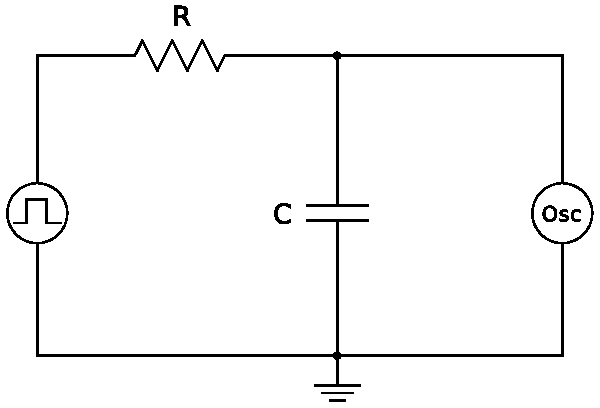
\includegraphics[width=100mm]{schema.pdf}
\end{SCfigure}

Facciamo notare che il circuito da noi utilizzato è alimentato da un'onda quadra che ci viene fornita dal generatore di forme d'onda. Questa configurazione è stata scelta al fine di sostituire un normale interruttore con il generatore di forme d'onda. Questo è stato fatto per poter ripetere ciclicamente il processo di carico e scarico del nostro condensatre.
La differenza di potenziale utilizzata è di $V\ped{0} \,=\, 1\,\si{\volt}$. Questa scelta è stata dettata dalla necessita di effettuare una rapida lettura del tempo caratteristico dall'oscilloscopio. Infine facciamo notare che abbiamo deciso di utilizzare una frequenza di $20\,\si{\hertz}$ per il generatore di funzioni d'onda al fine di ottenere un'immagine chiara e distinta dell'andamento della tensione in funzione del tempo sull'oscilloscopio.